
\section{Simulation Results}

In this section, we present simulation results that explore
the following performance aspects of our devised algorithm:
%
\begin{itemize}
\item  the execution time of the algorithm,
\item  the optimality gap for solving the $\ACONN$ and $\SCONN$ problems, and
\item  the effect of using relay nodes.
\end{itemize}

To explore the optimality gap of the devised algorithm, we have implemented
an exhaustive algorithm for computing exact solutions.
%
The algorithm works by generating all possible network states
of a given probabilistic network.
%
The exhaustive algorithm has a complexity that grows exponentially with
the number of nodes in the network. However, it can process a graph
with 10, or fewer, nodes in a reasonable time.
%
Both of the exhaustive algorithm, and our devised tree algorithm
are implemented in C++ with the use of STL (Standard Template Library)
container classes.


\nwline
{\bf Maximum Spanning Trees.}
To use our devised algorithm for obtaining lower bounds on $Conn(G,\nReq)$
of a given network, we need to select a spanning tree.
%
Ideally, one would prefer to use a spanning tree that gives the best
possible lower bound.
%
Currently, however, this latter problem appears to be an open problem.
%
In the absence of a known algorithm to compute such an optimum tree,
we resort to using a heuristic algorithm.
%
The algorithm works as follows.
%
We associate with each link $(x,y) \in E_G$ a probability, denoted $p(x,y)$,
of having the link $(x,y)$ present, given the locality sets $\loc(x)$ and
$\loc(y)$.
%
We then seek to compute a spanning tree with the highest possible
product of link probabilities.
%
This latter problem can be solved efficiently by using a standard minimum
spanning tree algorithm.
%
The results discussed utilizes such maximum spanning trees.


\nwline
{\bf Test Networks.}
%
For simplicity of constructing test networks and analyzing the obtained
results, we assume that all nodes have the same transmission range
$R_{tr}$, and we set the $E_G$ relation according to the Euclidean
distance between the involved nodes.

We have experimented with networks of different sizes in the range
[10,20] nodes where each node has a locality set in the range $[2,8]$
rectangles.
%
Here, we present selected results using the two networks in
Fig.~\ref{sim:g10}, denoted $G_{10}$, and
Fig.~\ref{sim:g10r}, denoted $G_{10,3}$.
The selected results are representative of the important findings
observed when using other networks.
%
The network $G_{10}$ has 10 sensor nodes, where $v[1]$ is the sink node.
%
As indicated in Fig.~\ref{sim:g10}, node locality sets vary in the range
$[3,6]$ locations where each location is a grid square of unit side length.
%
The figure illustrates a subset of links in $E_G$ that occur when 
$R_{tr}= 6.5$ units.
%
To avoid cluttering the diagram, we omit the $(x,y)$-coordinates of the
locality sets.
%
The network $G_{10,3}$ adds 3 relay nodes to $G_{10}$.
%
The exhaustive algorithm for computing exact connectivity deals only
with the links shown in $G_{10}$ and $G_{10,3}$ (some links may not
arise if $R_{tr} < 6.5$).
%
Solid lines in the figures indicate the links used in a maximum spanning tree.

     % ------------------------------
     %\begin{figure}[!ht]
     \begin{figure}[htbp]
     \begin{center}
     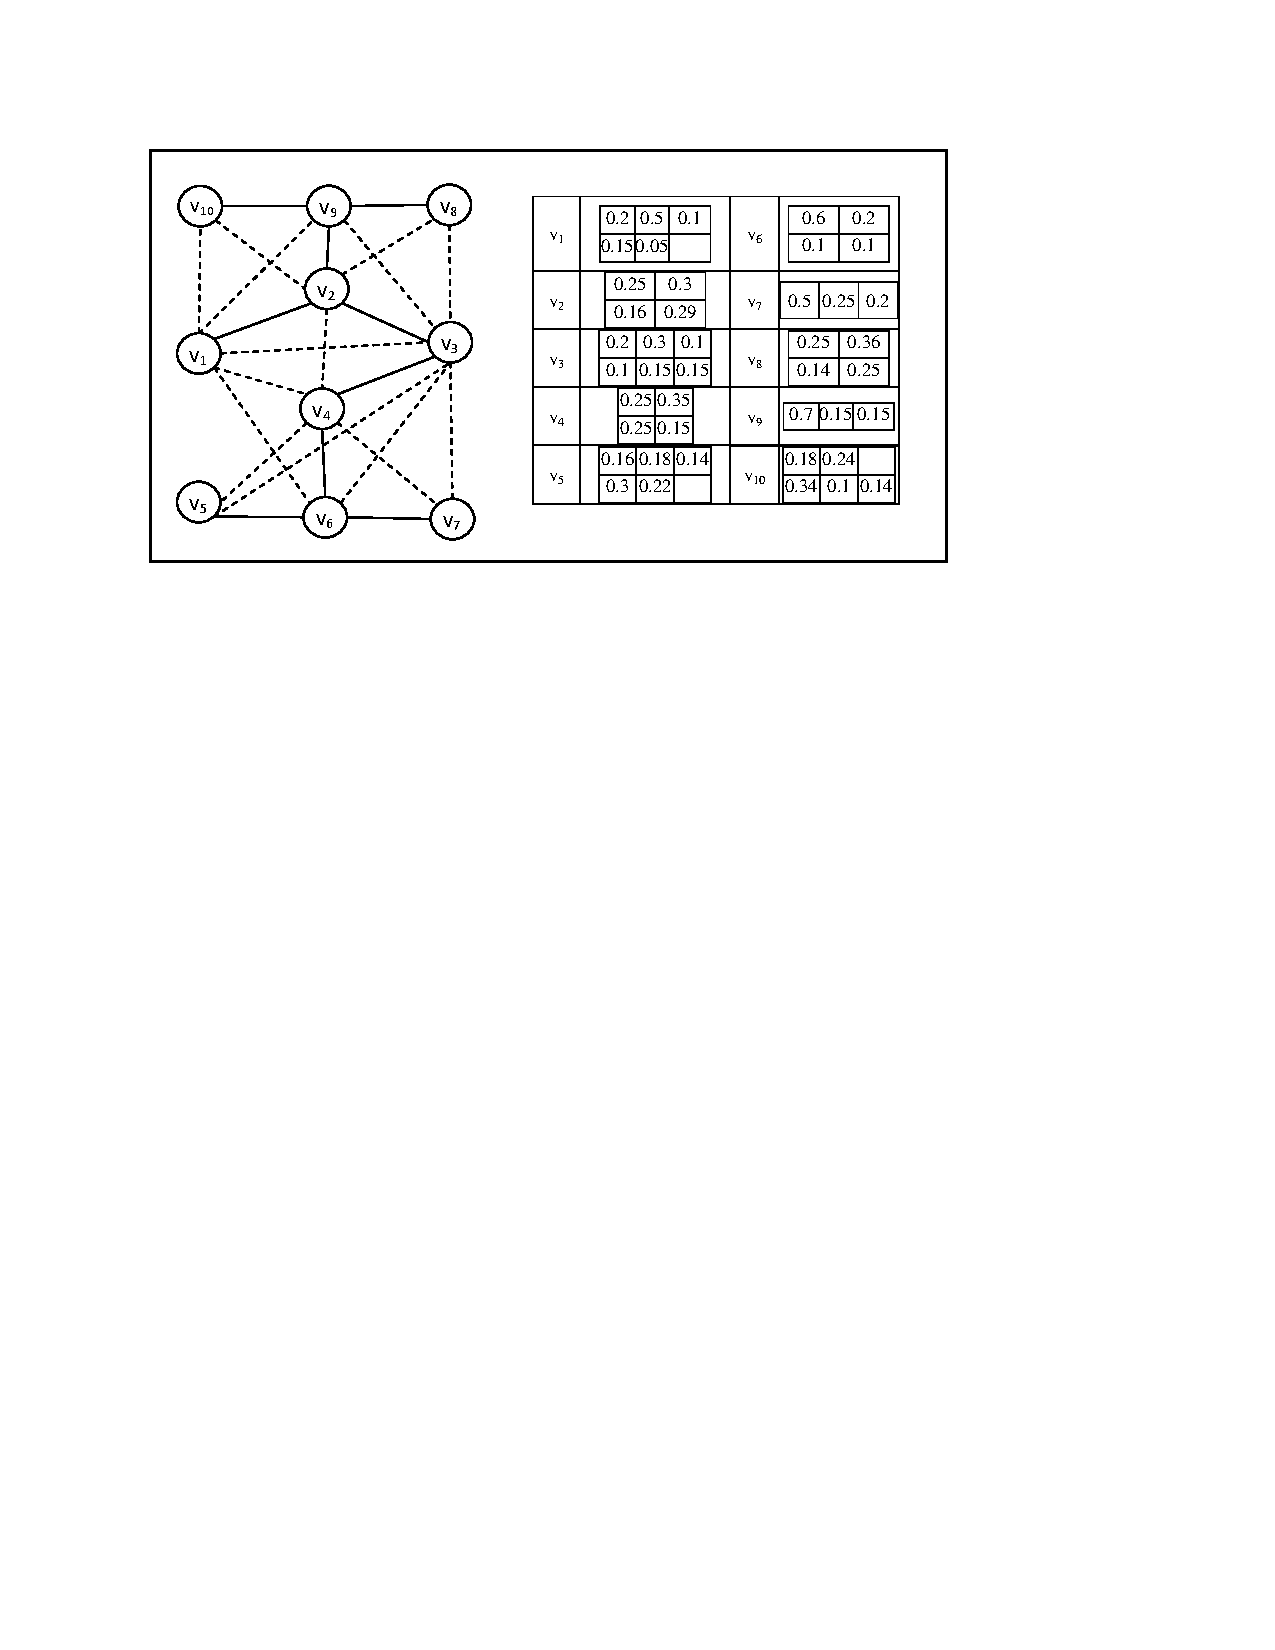
\includegraphics[width=3.3in]{g10.pdf}
     %
     % \caption{A probabilistic network on 10 nodes}
     \caption{The $G_{10}$ network}
     \label{sim:g10}
%\vspace*{-0.2in}
     \end{center}
     \end{figure}
     % ------------------------------
\vspace*{-0.2in}
     % ------------------------------
     %\begin{figure}[!ht]
     \begin{figure}[htbp]
     \begin{center}
     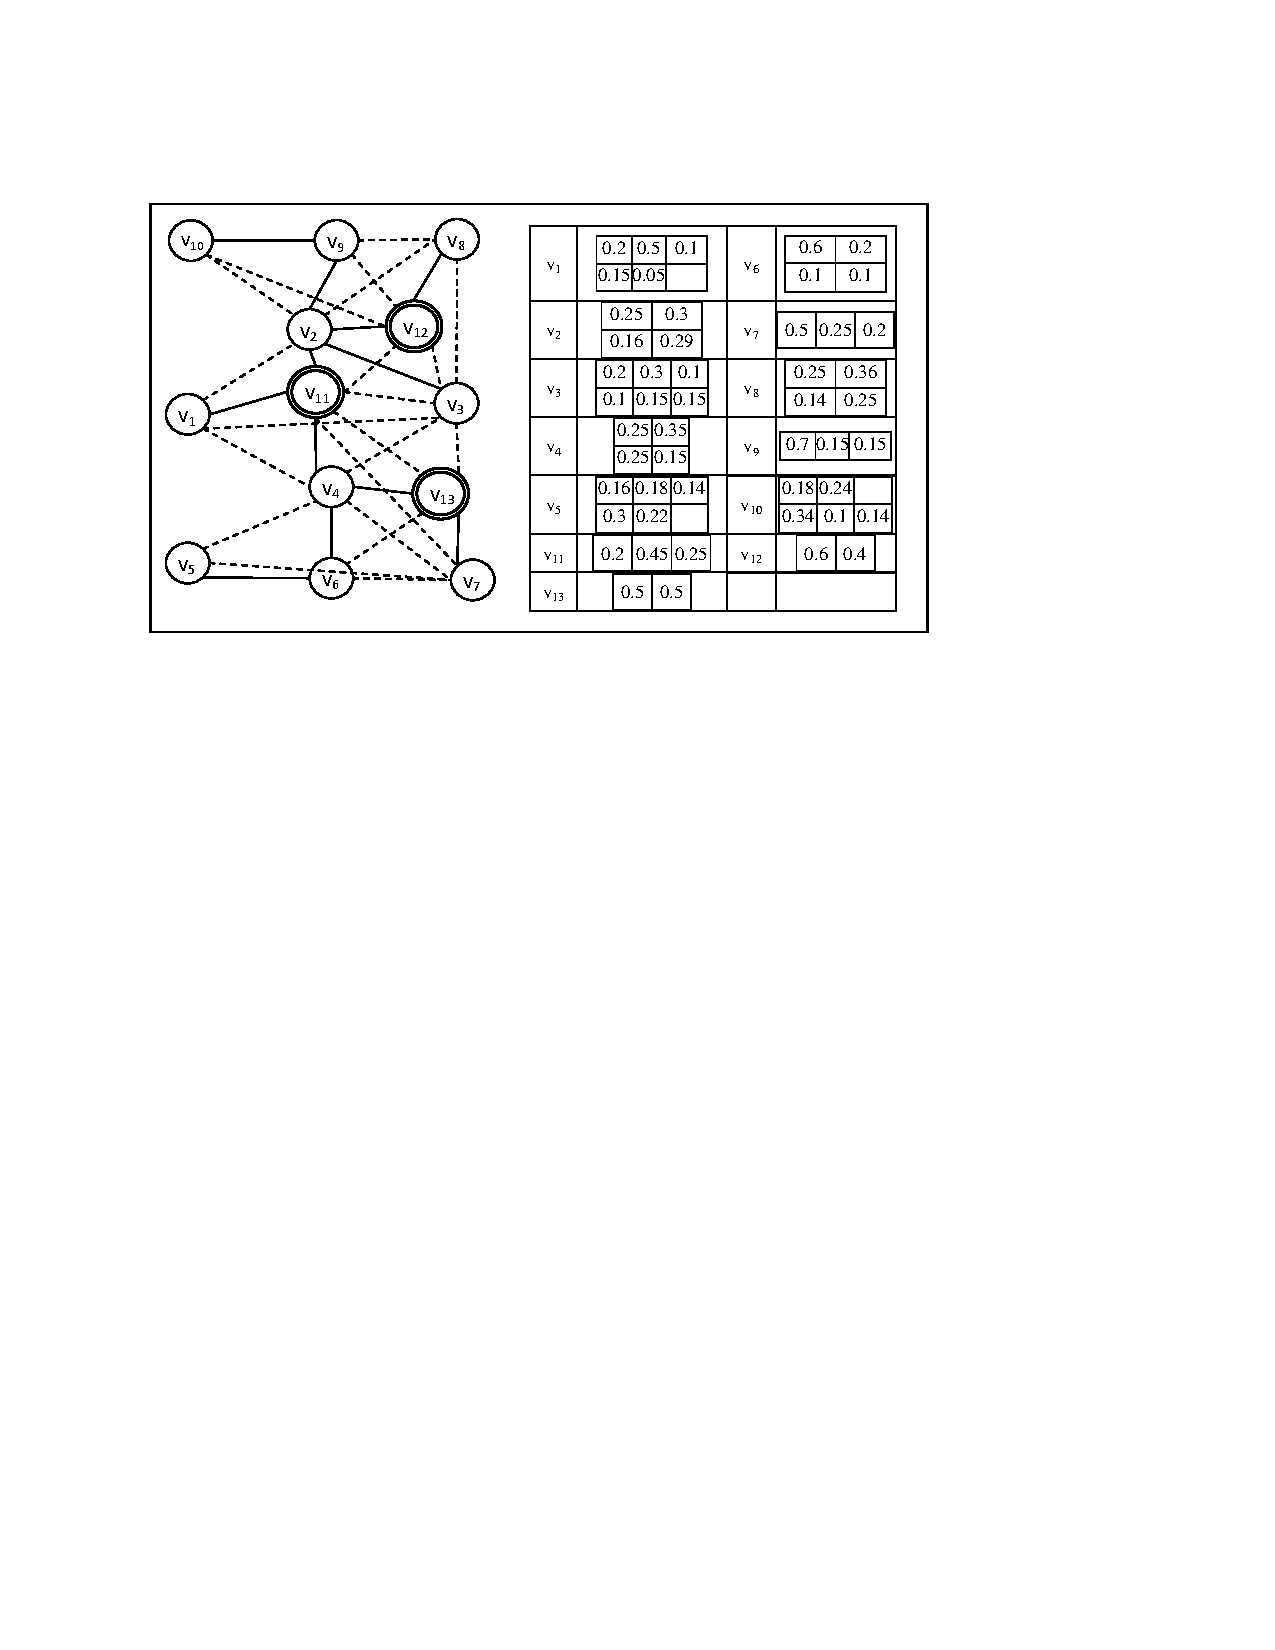
\includegraphics[width=3.3in]{g10-3r.pdf}
     %
     % \caption{A probabilistic network on 10 nodes and 3 relays}
     \caption{The $G_{10,3}$ network}
     \label{sim:g10r}
%\vspace*{-0.2in}
     \end{center}
     \end{figure}
     % ------------------------------
% ------------------------------

\nwline
{\bf 1. Running Time.}
The tree algorithm is empirically fast. The running time is typically
less than 50 millisec for the tested tree networks of size $\leq 20$ nodes.
In contrast, the exhaustive algorithm may require an hour to solve
a network of 10 nodes.

% ------------------------------

\noindent
     % ------------------------------
     %\begin{figure}[!ht]
     \begin{figure}[htbp]
     \begin{center}
     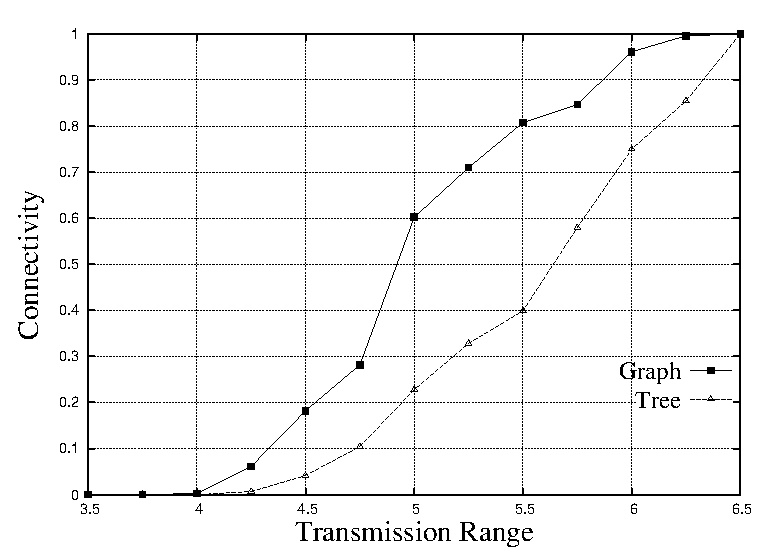
\includegraphics[width=3.0in]{conn-vs-trans.eps}
     % \caption{Exp-vs-size-pCom}
     \caption{Connectivity versus transmission range}
     \label{sim:conn:vs:trans}
%\vspace*{-0.2in}
     \end{center}
     \end{figure}
     % ------------------------------

{\bf 2. Tree bound versus exact solution for the $\ACONN$ problem.}
%
Fig.~\ref{sim:conn:vs:trans} illustrates the obtained results on $G_{10}$
when $R_{tr}$ varies in the range $[3.5,6.5]$ units.
%
Varying $R_{tr}$ in this range results in topologies with possibly
fewer links than shown in $G_{10}$.
%
When $R_{tr} \in [4.5,6.5]$, the ratio $Conn(G)/Conn(T)$ is found to be
in the range $[4.4,1]$. The ratio decreases monotonically as $R_{tr}$
increases.
%
The above finding suggests that the lower bound is more effective for
networks with good overall connectivity probability.
% ------------------------------

\noindent
     % ------------------------------
     %\begin{figure}[!ht]
     \begin{figure}[htbp]
     \begin{center}
     \includegraphics[width=3.0in]{conn-vs-nReq.eps}
     % \caption{Exp-vs-size-pSense}
     \caption{Connectivity versus $\nReq$}
     \label{sim:conn:vs:nreq}
%\vspace*{-0.2in}
     \end{center}
     \end{figure}
     % ------------------------------

{\bf 3. Tree bound versus exact solution for the $\SCONN$ problem.}
%
Fig.~\ref{sim:conn:vs:nreq} illustrates the obtained results on $G_{10}$
when $\nReq$ varies in the range $[1,10]$ nodes, and $R_{tr}= 6.5$.
%
The decreasing shape of the curves occur since increasing $\nReq$ results
in larger network states that arise with smaller probability.
%
When $\nReq$ varies in the range $[2,5]$, the ratio
$Conn(G,\nReq)/Conn(T,\nReq)$ is found to be in the range $[1.5,4.5]$.
%
The ratio deteriorates (to larger values) as $Conn(G,\nReq)$ takes small
values.
%
So, our finding here too is that the tree bound tends to be more useful
when the expected connectivity probability is relatively high.

% ------------------------------

\noindent
     % ------------------------------
     %\begin{figure}[!ht]
     \begin{figure}[htbp]
     \begin{center}
     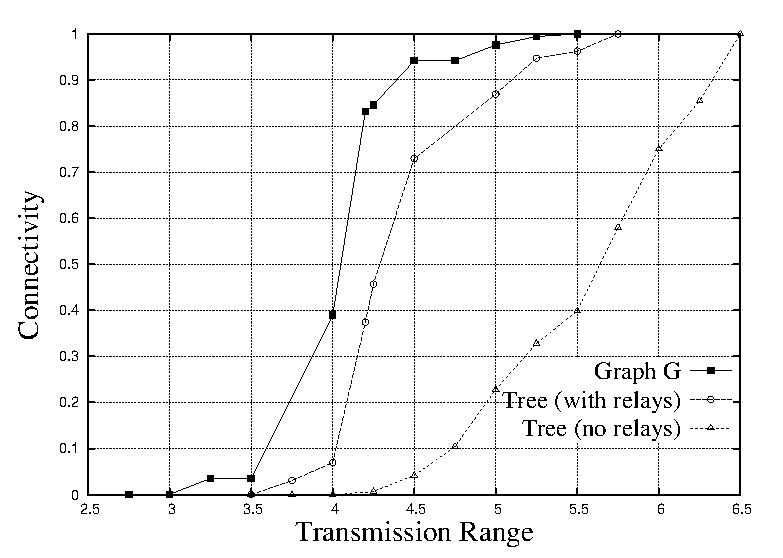
\includegraphics[width=3.0in]{conn-vs-trans-relay.eps}
     \caption{Effect of using relay nodes}
     \label{sim:conn:vs:trans:relay}
%\vspace*{-0.2in}
     \end{center}
     \end{figure}
     % ------------------------------

{\bf 4. Effect of adding relays.}
%
Deploying relay nodes can potentially increase the number of paths
from the sink node to many sensor nodes in the network.
%
Thus, the use of relay nodes can potentially improve the $Conn$ measures.
%
As it turns out, this positive effect is also reflected when using
a tree subnetwork.
%
This follows since relay nodes located in close proximity of a number
of sensor nodes can provide higher connectivity probability 
among the nodes than when removing them.
%
Fig.~\ref{sim:conn:vs:trans:relay} illustrates such positive effect
for the $\ACONN$ problem when $R_{tr}$ varies in the range $[2.5,6.5]$.
%
We have also encountered some unexpected cases where the tree bound
$Conn(T)$ of a spanning tree of a network with relays is higher
than $Conn(G)$ where $G$ is the corresponding network without relays.
%
Such findings support the positive role of using relays in UWSNs.


% ============================================================

% ------------------------------------------------------------
     % ------------------------------
%     \begin{figure*}[!ht]
%     \begin{center}
%         \subfloat[Exp-vs-size-pCom]
%         {
%          \includegraphics[width=2.2in]{exp-vs-width-pCom.eps}
%          \label{sim:exp:vs:size:pCom}
%         }
%         \iin{0.02}
         % ------------------------------
%         \subfloat[Exp-vs-size-pSense]
%         {
%          \includegraphics[width=2.2in]{exp-vs-width-pSense.eps}
%          \label{sim:exp:vs:size:pSense}
%         }
%         \iin{0.02}
         % ------------------------------
%         \subfloat[Exp-vs-Size-pCom-enhanced-cuts]
%         {
%          \includegraphics[width=2.2in]{exp-vs-size-pCom-enhanced-cuts.eps}
%          \label{sim:exp:vs:size:pCom:enhanced:cuts}
%         }
         % ------------------------------
%     \nwline
%         \subfloat[Exp-vs-Size-pSense-enhanced-cuts]
%         {
%          \includegraphics[width=2.2in]{exp-vs-size-pSense-enhanced-cuts.eps}
%          \label{sim:exp:vs:size:pSense:enhanced:cuts}
%         }
         % ------------------------------
%         \subfloat[Exp-vs-sink-location-LB]
%         {
%          \includegraphics[width=2.2in]{exp-vs-sink-location-LB.eps}
%          \label{sim:exp:vs:sink:location:LB}
%         }
         % ------------------------------
%         \subfloat[Exp-vs-Rjam-LB]
%         {
%          \includegraphics[width=2.2in]{exp-vs-Rjam-LB.eps}
%          \label{sim:exp:vs:Rjam:LB}
%         }
         % ------------------------------
%    \caption{Simulation Results}
%    \end{center}
%    \vspace{-0.3in}
%    \end{figure*}
    % ------------------------------

% ------------------------------------------------------------


